\documentclass[tikz,border=5pt]{standalone}
\usepackage[T1]{fontenc}
\usepackage{lmodern}
\usetikzlibrary{calc,backgrounds}
\definecolor{navy}{HTML}{26384A}
\definecolor{blue}{HTML}{2F80C1}
\definecolor{teal}{HTML}{168C82}
\definecolor{orange}{HTML}{BD7914}
\definecolor{purple}{HTML}{7961A8}
\definecolor{red}{HTML}{C75450}
\tikzset{panel/.style={draw=#1!65,fill=#1!4,line width=.8pt,
 rounded corners=3mm,minimum width=65mm,minimum height=52mm,inner sep=0pt},
 title/.style={font=\rmfamily\bfseries\fontsize{10}{12}\selectfont,text=#1,anchor=north west},
 row/.style={font=\rmfamily\fontsize{9}{10.5}\selectfont,text=navy,
 anchor=north west,align=left,text width=58mm,inner sep=0pt},
 spoke/.style={line width=1.6pt,draw=#1!65}}
\newcommand{\optionrow}[4]{\node[row] at ([xshift=3.5mm,yshift=-#2mm]#1.north west)
 {\textbf{#3}\\#4};}
\begin{document}
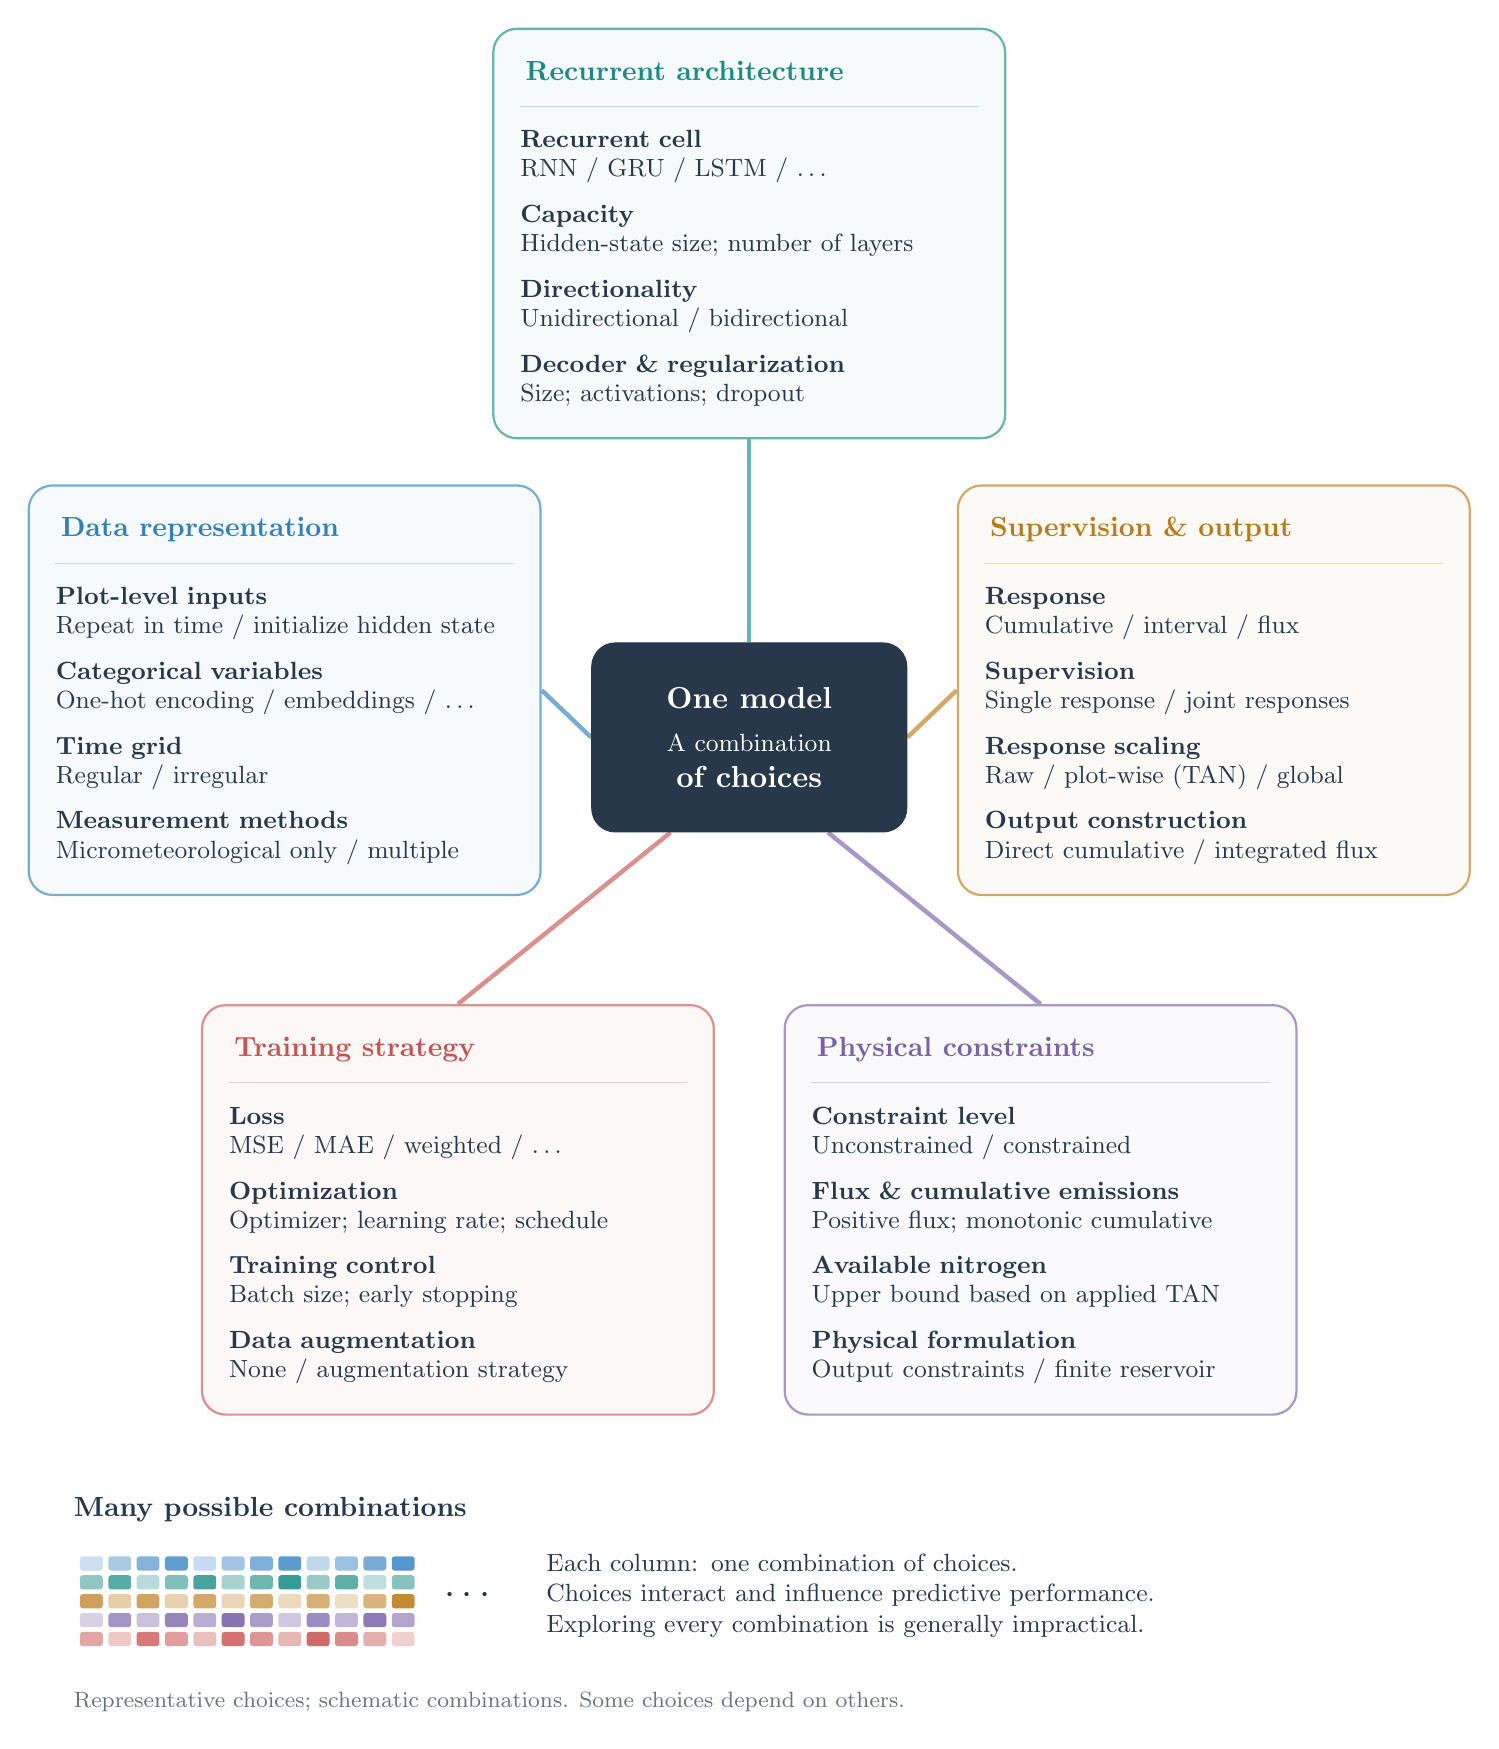
\begin{tikzpicture}[x=1mm,y=1mm]
\node[panel=teal] (architecture) at (0,68) {};
\node[panel=blue] (data) at (-59,10) {};
\node[panel=orange] (output) at (59,10) {};
\node[panel=red] (training) at (-37,-56) {};
\node[panel=purple] (physics) at (37,-56) {};
\foreach \name/\colour/\label in {
 architecture/teal/Recurrent architecture,data/blue/Data representation,
 output/orange/Supervision \& output,training/red/Training strategy,
 physics/purple/Physical constraints}{
 \node[title=\colour] at ([xshift=3mm,yshift=-3mm]\name.north west) {\label};
 \draw[\colour!30] ([xshift=3.5mm,yshift=-10mm]\name.north west)
 -- ([xshift=-3.5mm,yshift=-10mm]\name.north east);
}
\optionrow{architecture}{13}{Recurrent cell}{RNN / GRU / LSTM / \ldots}
\optionrow{architecture}{22.5}{Capacity}{Hidden-state size; number of layers}
\optionrow{architecture}{32}{Directionality}{Unidirectional / bidirectional}
\optionrow{architecture}{41.5}{Decoder \& regularization}{Size; activations; dropout}
\optionrow{data}{13}{Plot-level inputs}{Repeat in time / initialize hidden state}
\optionrow{data}{22.5}{Categorical variables}{One-hot encoding / embeddings / \ldots}
\optionrow{data}{32}{Time grid}{Regular / irregular}
\optionrow{data}{41.5}{Measurement methods}{Micrometeorological only / multiple}
\optionrow{output}{13}{Response}{Cumulative / interval / flux}
\optionrow{output}{22.5}{Supervision}{Single response / joint responses}
\optionrow{output}{32}{Response scaling}{Raw / plot-wise (TAN) / global}
\optionrow{output}{41.5}{Output construction}{Direct cumulative / integrated flux}
\optionrow{training}{13}{Loss}{MSE / MAE / weighted / \ldots}
\optionrow{training}{22.5}{Optimization}{Optimizer; learning rate; schedule}
\optionrow{training}{32}{Training control}{Batch size; early stopping}
\optionrow{training}{41.5}{Data augmentation}{None / augmentation strategy}
\optionrow{physics}{13}{Constraint level}{Unconstrained / constrained}
\optionrow{physics}{22.5}{Flux \& cumulative emissions}{Positive flux; monotonic cumulative}
\optionrow{physics}{32}{Available nitrogen}{Upper bound based on applied TAN}
\optionrow{physics}{41.5}{Physical formulation}{Output constraints / finite reservoir}
% All five families contribute to one model; no imposed sequence.
\node[draw=navy,fill=navy,rounded corners=3mm,text=white,
 minimum width=40mm,minimum height=24mm,align=center,
 font=\rmfamily\bfseries\fontsize{11}{13}\selectfont] (model) at (0,4)
 {One model\\[1mm]\normalfont\rmfamily\fontsize{9}{11}\selectfont
 A combination\\of choices};
\begin{scope}[on background layer]
 \draw[spoke=teal] (architecture.south) -- (model.north);
 \draw[spoke=blue] (data.east) -- (model.west);
 \draw[spoke=orange] (output.west) -- (model.east);
 \draw[spoke=red] (training.north) -- ([xshift=-10mm]model.south);
 \draw[spoke=purple] (physics.north) -- ([xshift=10mm]model.south);
\end{scope}
% Each mosaic column represents a combination of the five choice families.
\node[anchor=west,text=navy,font=\rmfamily\bfseries\fontsize{10}{12}\selectfont]
 at (-87,-94) {Many possible combinations};
\foreach \col in {0,...,11}{
 \foreach \row/\colour in {0/blue,1/teal,2/orange,3/purple,4/red}{
  \pgfmathtruncatemacro{\shade}{25+mod(\col*17+\row*23+\col*\row*7,65)}
  \fill[\colour!\shade,rounded corners=.35mm]
   ({-85+\col*3.6},{-100-\row*2.4}) rectangle ++(2.9,-1.8);
 }}
\node[anchor=west,text=navy,font=\rmfamily\Large] at (-40,-105) {$\cdots$};
\node[anchor=west,text=navy,align=left,text width=113mm,
 font=\rmfamily\fontsize{9}{11}\selectfont] at (-27,-105)
 {Each column: one combination of choices.\\
 Choices interact and influence predictive performance.\\
 Exploring every combination is generally impractical.};
\node[anchor=north west,text=navy!70,align=left,
 font=\rmfamily\fontsize{8}{9.5}\selectfont] at (-87,-116)
 {Representative choices; schematic combinations. Some choices depend on others.};
\end{tikzpicture}
\end{document}
